% !TEX root = ../notes.tex

% ================  (Interactive) Visualization ==============

\section{Supervised Learning}

%=============================================
\subsection{Introduction to Machine Learning}

The term {\bf Machine Learning} cannot be defined better than \href{https://en.wikipedia.org/wiki/Arthur\_Samuel}{Arthur Samuel}'s definition: ``{\it Field of study that gives computers the ability to learn without being explicitly programmed.}''. The idea behind Machine Learning is to use the computers to apply statistical and optimization algorithms to \emph{automatically} identify pattern in data and/or classify them. A \href{http://www.r2d3.us/visual-intro-to-machine-learning-part-1/}{beautiful introduction to Machine Learning} will speak more than thousand words. At the end we can simply say that Machine Learning is born because we are \textbf{lazy} and we let the machine do the ``work'' for us. 
\\\\
In Machine Learning, we can separate the algorithms either by the \emph{learning style} (Supervised vs Unsupervised vs Semi-Supervised learning) or by their \emph{similarity}. In the next part of this chapter, we first give an introduction to Supervised and Unsupervised learning and then we go deeper into the Supervised Learning. If you want to become a Machine Learning Master, you should have a look \href{http://machinelearningmastery.com/}{here}.

%=============================================
\subsubsection{Characteristics of Classification Methods} 

When we use Machine Learning methods we are expecting good predictions. But it is not the only important aspect of the Machine Learning methods. The following list gives some very important aspects for these methods:

\begin{itemize}
\item \textbf{Predictive accuracy}
\item \textbf{Speed and scalability} 
  \begin{itemize}
   \item Time to build the model
   \item Time to use the model
   \item In memory vs Disk processing
  \end{itemize}
\item \textbf{Robustness}
  \begin{itemize}
   \item Handling noise
   \item Handling outliers
   \item Handling missing values
  \end{itemize}
\item \textbf{Interpretability}
  \begin{itemize}
   \item Understand the model and its decisions (black box vs white box)
   \item Compactness of the model
  \end{itemize}
\end{itemize}

%=============================================
\subsubsection{Supervised vs Unsupervised Learning}

In Table \ref{tab:sup-unsup} we give some differences/similarities between Supervised and Unsupervised Learning. The main difference to remember is that for Supervised learning, we use a training data with known labels and we test it on a test data without labels. For Unsupervised learning we do not have any labels. We are just trying to simplify/cluster the samples.

\begin{table}[h!]
  \centering
  \begin{tabular}{m{2cm}||m{5.5cm}|m{5.5cm}}
    & Supervised & Unsupervised \\ \hline\hline
    Variables & Samples $X$ and labels $y$ & Samples $X$ \\ \hline
    Learning & Function $y = f(X)$ relate samples and labels. We would like to ``learn'' $f$ and evaluate it on new data. & We want to compute a function $y = f(X)$ to give a \emph{simpler} representation of the samples X. \\ \hline
    Discrete \newline labels & {\bf Classification} & {\bf Clustering} \\ \hline
    Continuous labels & Regression & Matrix factorization, Kalman filtering, Unsupervised neural networks \\ \hline 
    Examples & 
	      $\bullet$ Is this image a cat, dog, car, house? \newline
	      $\bullet$ How would this user score that restaurant? \newline
	      $\bullet$ Is this email spam? \newline
	      $\bullet$ Is this blob a supernova?
	     &
	      $\bullet$ Cluster some hand-written digit data into 10 classes. \newline
	      $\bullet$ What are the top 20 topics in Twitter right now? \newline
	      $\bullet$ Find and cluster distinct accents of people in Lausanne
            \\ \hline
    Techniques & 
	      $\bullet$ k Nearest Neighbors \newline
	      $\bullet$ Na\"ive Bayes \newline
	      $\bullet$ Linear + Logistic Regression \newline
	      $\bullet$ Support Vector Machines \newline
	      $\bullet$ Random Forests \newline
	      $\bullet$ Neural Networks
	    &
	      $\bullet$ Clustering \newline
	      $\bullet$ Topic Models \newline
	      $\bullet$ Hidden Markov Models
	    \\ \hline
  \end{tabular}
  \label{tab:sup-unsup}
  \caption{Summary of the differences between Supervised and Unsupervised learning.}
\end{table}

%=============================================
\subsection{More details on Supervised Learning}

%=============================================
\subsubsection{Predicting from Samples}

The \textbf{samples} are most of the time a subset of an infinite population. We are most interested in a model that can {\bf describe the whole population} but since we only have access to a \emph{sample} of it, it is not possible. Therefore we train on a training sample $D$ and we denote the model found by $f_D(X)$, $X$ being the features.
Most of the datasets are \textbf{samples} from an infinite population, \emph{i.e.} a subset of an \textbf{infinite} dataset. We would like to model the \textbf{whole population}, but only have access to a sample of it. So, we train on a training sample called $D$ and we denote the model as $f_D(X)$ where $X$ are the features and $y=f_D(X)$ the predictions.

%=============================================
\subsubsection{Bias and Variance}

The data-generated model $f_D(X)$ is a \textbf{statistical estimate} of the true function $f(X)$ (function working for the whole population). Therefore the model is subject to bias and variance. 
\\
The \textbf{Bias} is defined as the \emph{expected difference} between the prediction of a model $f_D(X)$ and the true labels $y$:
\[
 \textrm{Bias} = \mathbb{E}\left[ f_D(X)-y\right]
\]
\\
The \textbf{Variance} is defined as:
\[
 \textrm{Variance} = \mathbb{E}\left[\left(f_D(X) - \overline{f}(X)\right)^2\right]
\]
where $\overline{f}(X) = \mathbb{E}\left[f_D(X)\right]$ being the average prediction on X.

Bias and Variance are very useful to understand if you're doing something wrong. Thus it is important to understand what you are doing and not just applying ``black-boxed'' algorithms.

\textbf{Tradeoff between Bias and Variance}
\\\\
The \href{http://scott.fortmann-roe.com/docs/BiasVariance.html}{tradeoff between bias and variance} is due to model complexity, see Figure \ref{fig:simple_complex}.
\begin{itemize}
 \item \textbf{Complex models}: Many parameters, usually lower bias but higher variance
 \item \textbf{Simple models}: Few parameters, higher bias but lower variance.
\end{itemize}
\begin{figure}[H] %----------- Graph ---------------------
\centerline{
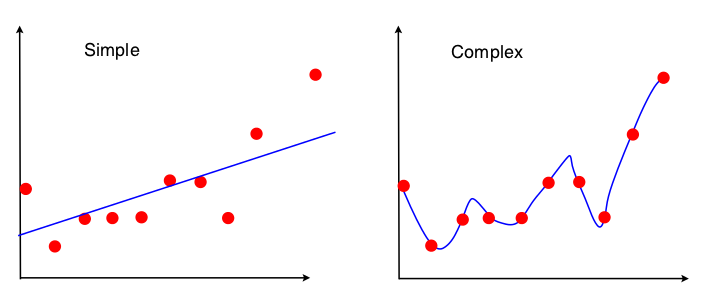
\includegraphics[width=13cm]{img/07/simple_complex}
}
\caption{\label{fig:simple_complex} 
Illustrations of a simple model and a complex model on the same data.
}
\end{figure}


For example, a linear model can only fit a straight line. A high degree polynomial can fit complex curves. Therefore this polynomial will work very well with the samples but not that well with the whole population. Thus a high variance is expected.
\\\\
In order to take into account this tradeoff, we introduce the total expected error is 
\[
 \textrm{Bias}^2 + \textrm{Variance}
\]
This error {\bf balance} the contributions of the variance and the bias. 

\begin{figure}[H] %----------- Graph ---------------------
\centerline{
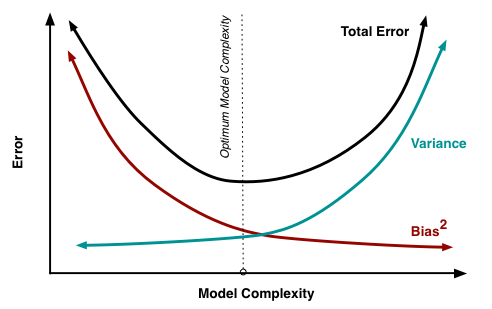
\includegraphics[width=10cm]{img/07/biasvariance}
}
\caption{\label{BV} 
Illustration of the model complexity and the Bias Variance tradeoff. The optimum model complexity is when the total error is minimized.
}
\end{figure}
When the Bias and the Variance are unbalanced, we use the terms:
\begin{itemize}
 \item {\bf overt-fitting} when the \emph{Variance} strongly dominates. (Too much variation between models)
 \item {\bf under-fitting} when the \emph{Bias} strongly dominates. (The models are not fitting the data well enough)
\end{itemize}


%=============================================
\subsection{k-Nearest Neighbors}

The kNN algorithm is a well known method used for classification and regression. The input consists simply of the k closest training examples. The idea of the kNN algorithm is to find the k nearest neighbors of an input using a specific metric. Once we found them, we can give the label of the new input such that it corresponds to the most used label in the neighbors. Figure \ref{fig:knn} shows an example with cats and other animals.

\begin{figure}[H] %----------- Graph ---------------------
\centerline{
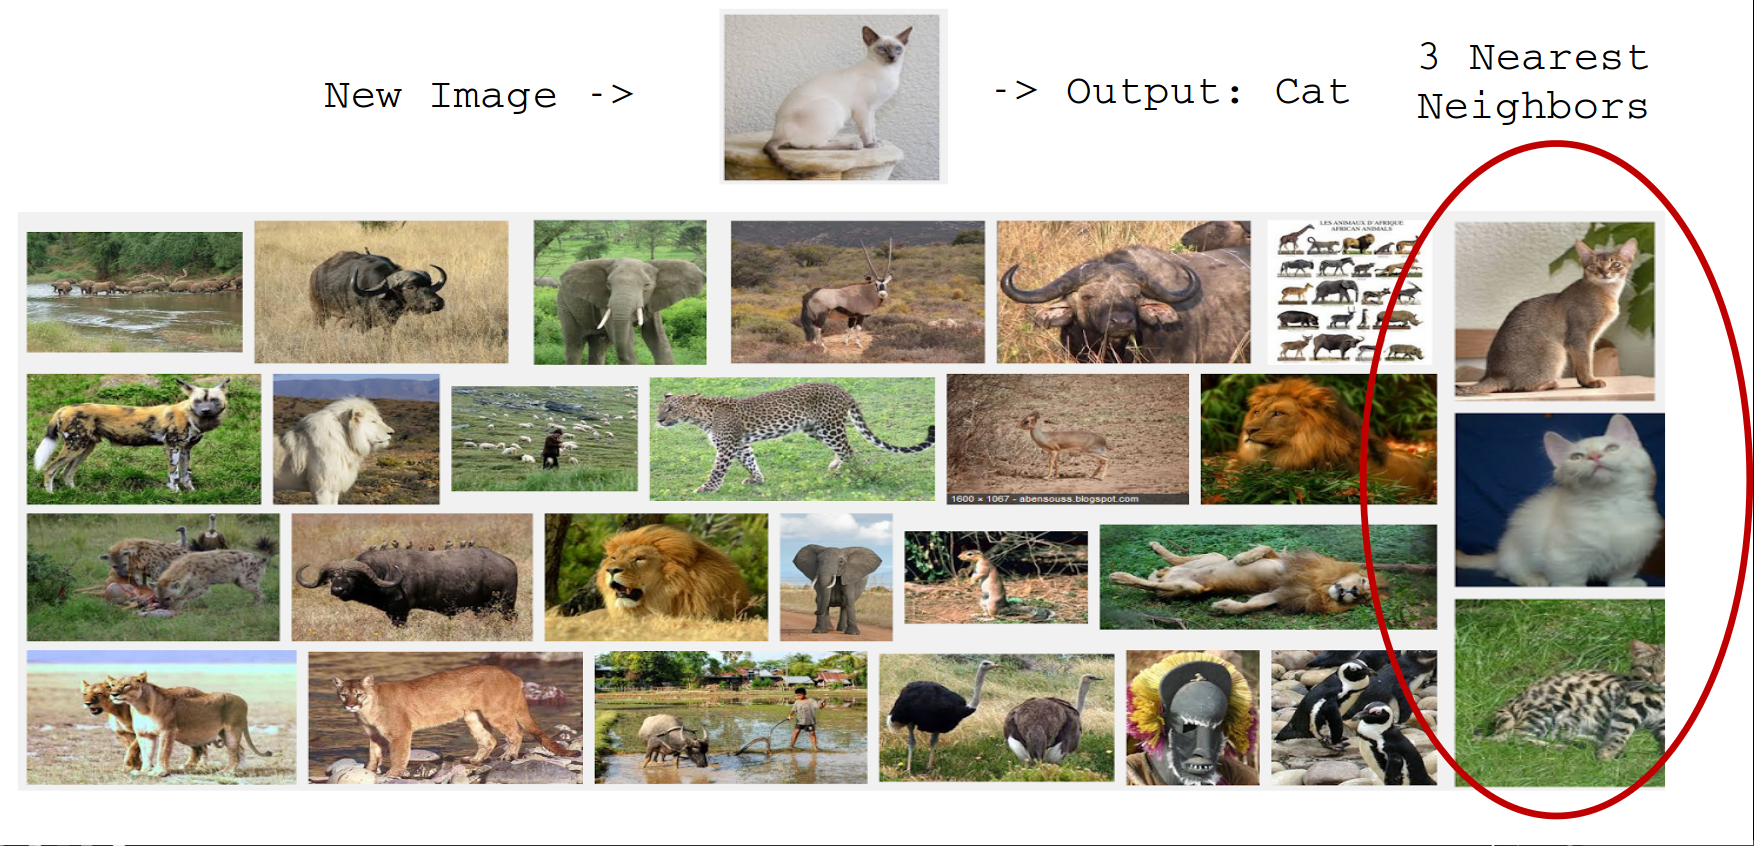
\includegraphics[width=13cm]{img/07/knn}
}
\caption{\label{fig:knn} 
Illustration of the kNN algorithm.
}
\end{figure}
\newpage
However this very simple algorithm has one issue: the Data {\bf is} the Model. This implies:
\begin{itemize}
 \item No training needed.
 \item The accuracy generally improves with more data.
 \item Matching is simple and fairly fast if data fits in memory. (Can be run off disk)
\end{itemize}
Normally, the only parameter is $k$, the number of neighbors. But two other choices are important:
\begin{itemize}
 \item Weighting of neighbors (e.g. inverse distance)
 \item Similarity metric.
\end{itemize}

%=============================================
\subsubsection{kNN Flavors}
The kNN algorithm can be used both for regression and classification. Table \ref{tab:knn} gives the similarities/differences of the kNN algorithm for regression and classification.
\begin{table}[h!]
 \centering
 \begin{tabular}{p{7cm}|p{7cm}}
  Classification & Regression \\ \hline \hline
  The model is $y=f(X)$ where $y$ is from a discrete set (labels). & The model is $y=f(X)$ where $y$ is a real value. \\ \hline
  Given $X$, we compute $y$ being the majority vote of the k nearest neighbors. & Given $X$, we compute $y$ being the average value of the k nearest neighbors. \\ \hline
  We can also use a weighted vote of the neighbors. & We can also use a weighted average of the neighbors.
 \end{tabular}
 \label{tab:knn}
 \caption{kNN algorithm used for classification and regression: Differences and similarities. Usually, the weight function is the inverse distance. 
}
\end{table}

%=============================================
\subsubsection{kNN distance measures}
For the kNN algorithm, we need to use a distance between the neighbors. The choice of the distance function can be very different depending on what you are looking for. We give here some examples:
\begin{description}
 \item[Euclidean distance] Simple, fast to compute.
 \[
  d(x,y) = ||x-y||
 \]

 \item[Cosine Distance] Good for documents, images, etc.
 \[
  d(x,y) = 1- \frac{x\cdot y}{||x||||y||}
 \]

 \item[Jaccard Distance] For set data
 \[
  d(X,Y) = 1 - \frac{|X \cap Y|}{|X \cup Y|}
 \]

 \item[Hamming Distance] For string data
 \[
  d(x,y) = \sum_{i=1}^{n} \left( x_i \neq y_i \right)
 \]
 \item[Manhattan Distance] Coordinate-wise distance
 \[
  d)x,y) = \sum_{i=1}^n |x_i - y_i|
 \]
 \item[Edit Distance] For strings, especially genetic data. See on \href{https://en.wikipedia.org/wiki/Edit\_distance}{Wikipedia} for more information.
 \item[Mahalanobis Distance] Normalized by the sample covariance matrix -- unaffected by coordinate transformations. 
 \[
  d(x,y) = \sqrt{\left(x-y\right)^TS^{-1}\left(x-y\right)}
 \]
 where $S$ is the covariance matrix.
\end{description}

%=============================================
\subsubsection{Choosing k}

If we choose a {\bf small k}, we will see a low bias but high variance. Firgure \ref{fig:knn_k1} shows whats happens with two different samples if we choose a small k.

\begin{figure}[H] %----------- SubGraph ---------------------
\centerline{
\subfigure{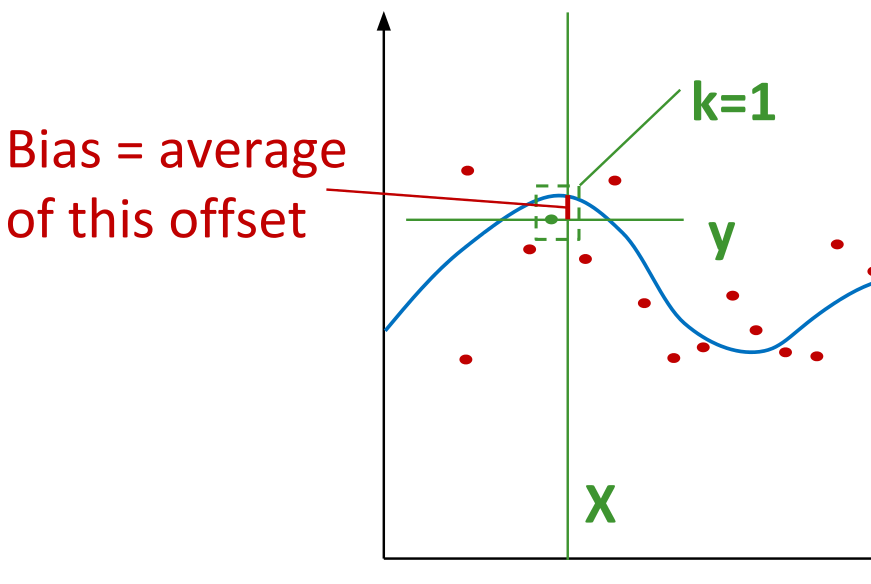
\includegraphics[width=7cm]{img/07/k1_original}}\quad
\subfigure{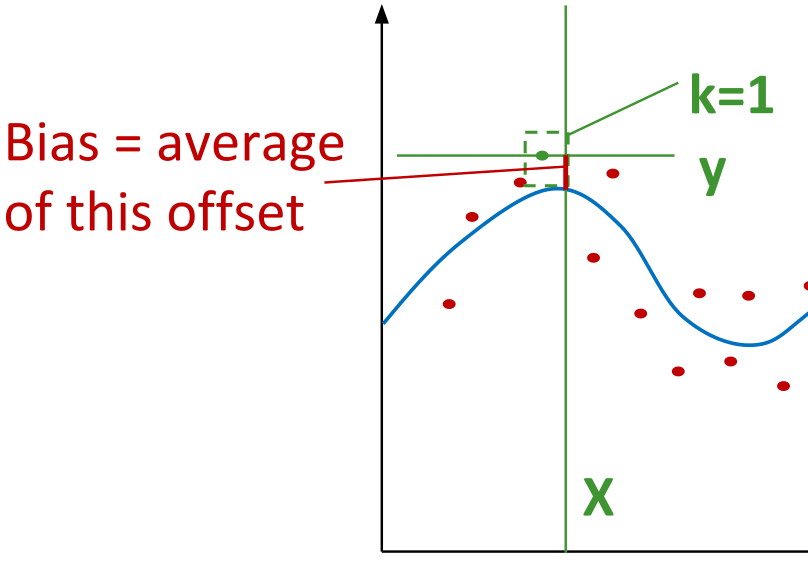
\includegraphics[width=7cm]{img/07/k1_diff}} 
}
\caption{\label{fig:knn_k1} 
Test on two different samples of the kNN algorithm with k=1.
}
\end{figure}

On the other hand if we choose a {\bf large k}, we will see a high bias but low variance. Firgure \ref{fig:knn_k8} shows whats happens with two different samples if we choose a large k.

\begin{figure}[H] %----------- SubGraph ---------------------
\centerline{
\subfigure{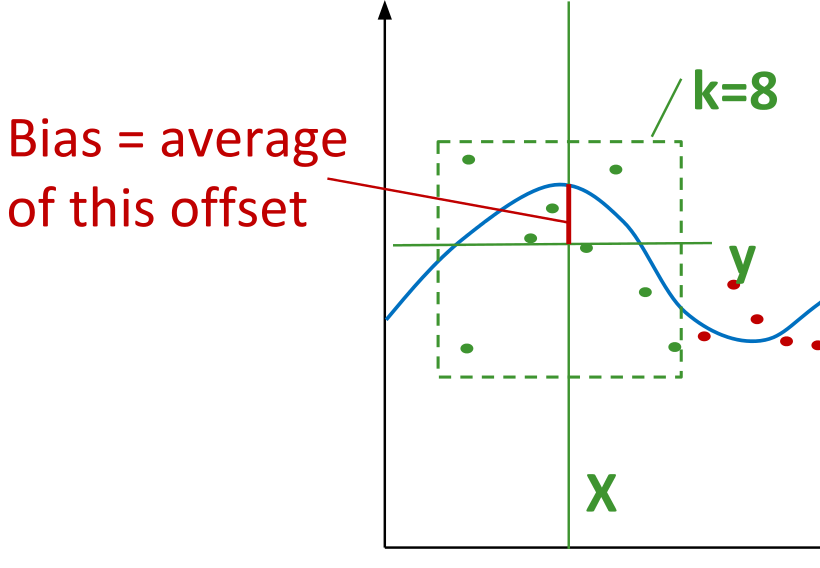
\includegraphics[width=7cm]{img/07/k8_original}}\quad
\subfigure{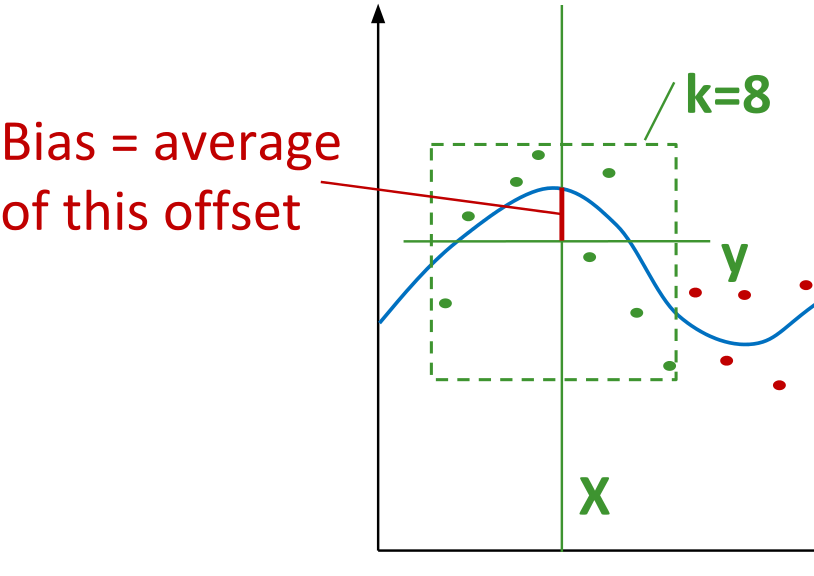
\includegraphics[width=7cm]{img/07/k8_diff}} 
}
\caption{\label{fig:knn_k8} 
Test on two different samples of the kNN algorithm with k=8.
}
\end{figure}

\textbf{In practice}
\\
\begin{description}
 \item[Use cross-validation!] Break data into train, validation and test subsets. For example, you can choose a 60-20-20 \% random split.
 \item[Predict] For each point in the validation set, predict using the k-Nearest neighbors from the training set. Measure the error rate (classification) or the squared error (regression)
 \item[Tune] Try different values of k, and use the one that gives minimum error on the validation set.
 \item[Evaluate] test on the test set to measure performance.
\end{description}

%=============================
\subsubsection{kNN and the curse of dimensionality}

The curse of dimensionality refers to phenomena that occur in high dimensions, from hundreds to millions, that do not occur in low-dimensional space. Data in high dimensions are much sparser than data in low dimensions. That means there are less points that are very close in the feature space. For example, the Euclidean distance scales as $\sqrt{N}$ with $N$ being the dimension. Thus it is quite surprising that kNN works even in high dimensions. 

Luckily data are not random points in a high-dimensional cube. They live in {\bf dense clusters} and near {\bf much lower-dimensional surfaces}. Therefore, we can reduce the feature space in many different way to see the clusters appear.

Even if the Euclidean distance between two point is large they can be very \emph{similar}. For example documents with the same few dominant words (with \href{https://en.wikipedia.org/wiki/Tf-idf}{tf-idf} weighting) are likely to be on the same topic.

%=============================
\subsection{Decision Tree}

Decision Tree (DT) is a basic classifier acting like a \textbf{flow-chart having a tree structure}. It's constructed following a top-down approach in which, at each node, the data are split on one of their attribute. The prediction are obtained by following the "if-else" statement of each node and is given by the leaves, once the whole tree is traversed.
\\\\
The only way to score a DT is by counting the number of right elements it predicts on the test set, since the prediction are not "weighted" by a probability of correctness.

\begin{figure}[H] %----------- SubGraph ---------------------
\centerline{
\subfigure{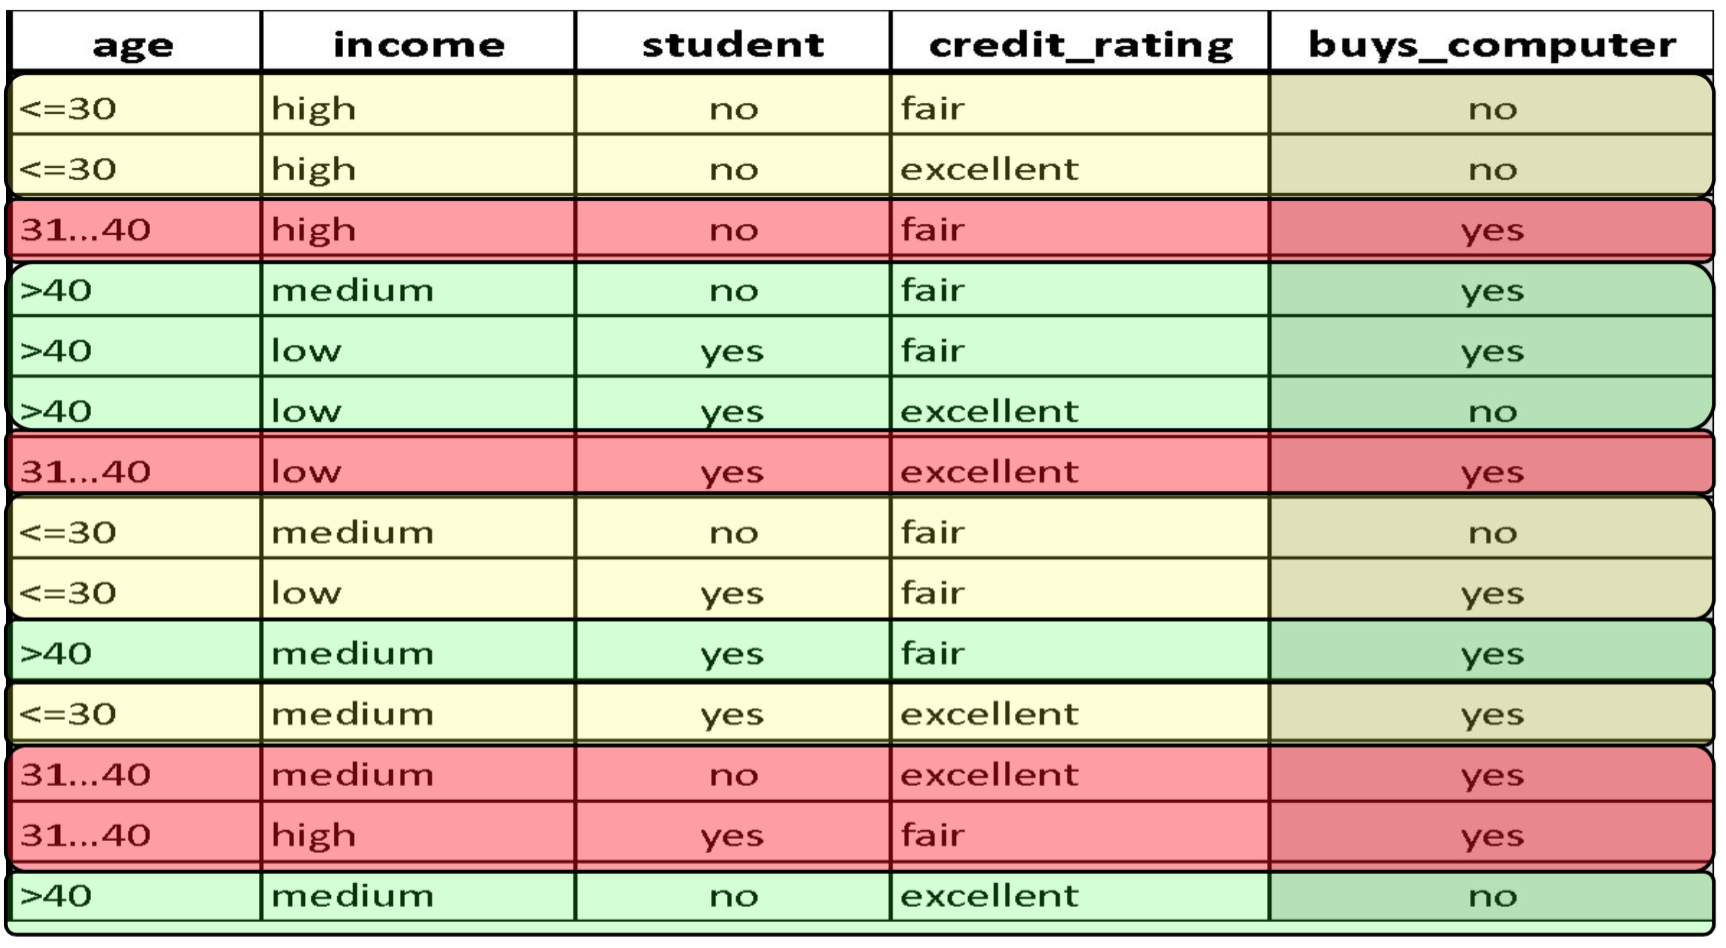
\includegraphics[width=5.5cm]{img/07/DT1}}
\subfigure{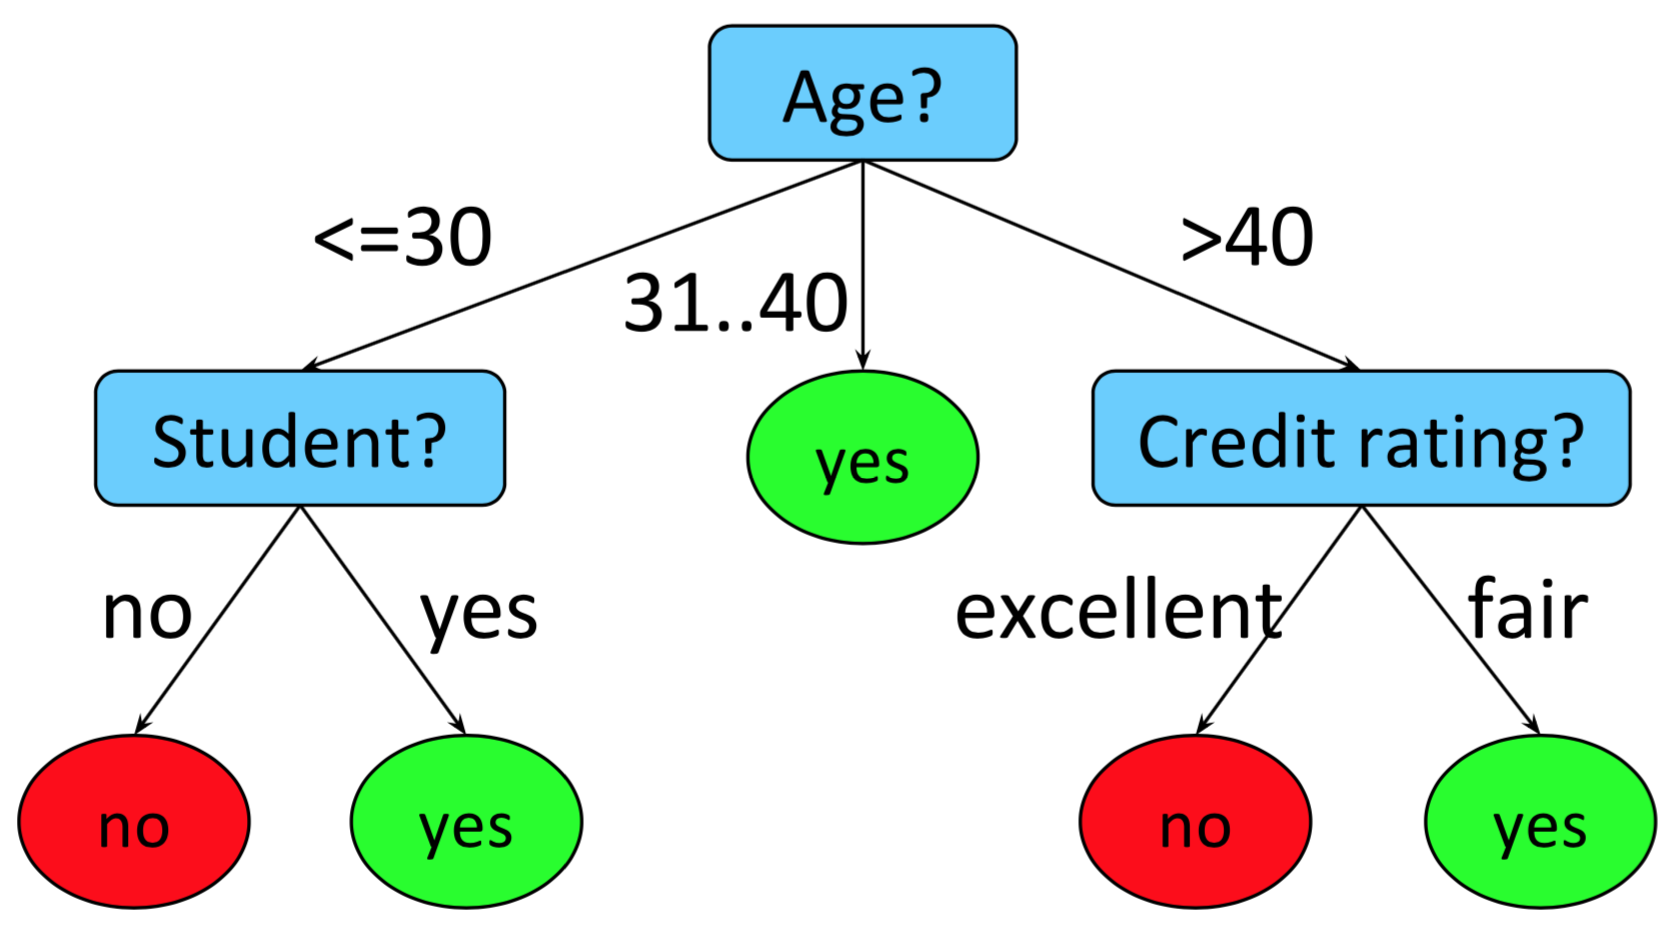
\includegraphics[width=5.5cm]{img/07/DT2}} 
}
\caption{\label{DT} 
Dataset and the Decision Tree related to it.
}
\end{figure}

\textbf{Construction} (Top-down, divide-and-conquer strategy.)
\begin{enumerate}
  \item At the beginning, all the data belong to the node
  \item Recursively, the (sub)sets are partitioned on their most discriminative attribute (see section \ref{sec:selection})
  \item Stop when:
  \begin{itemize}
  	\item A node only contains same labeled data, stop and make it a leaf labeled the same.
  	\item No more attributes left, assigne the most present
  	\item No more data left.
  	\item (A thershold has been defined and is reached)
  \end{itemize}
\end{enumerate}

The DT will continue to add attributes to its decision process until no ones left. As it increases its precision (and then its depth), it starts overfiting the model. A threshold can be defined to stop the construction process earlier and limit this effect. 

\begin{figure}[H]%---------------FIG--------------
 \centering
 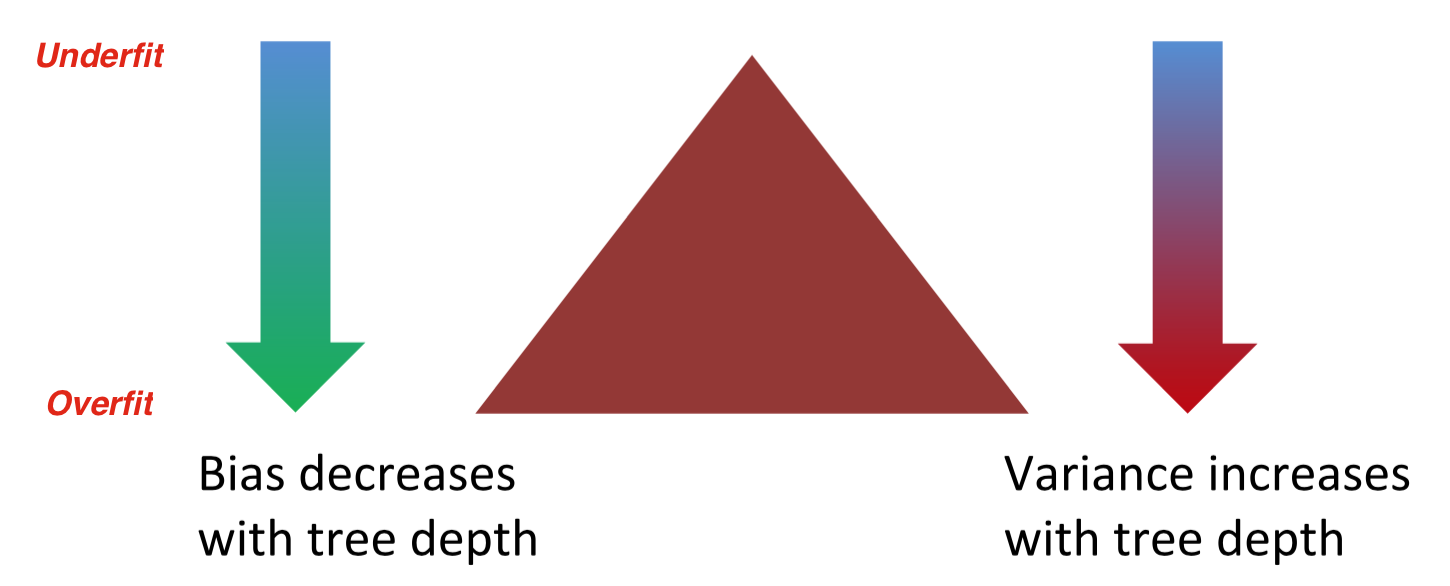
\includegraphics[width=10cm]{./img/07/bias_variance_DT.png}
 \caption{\label{pic:bias_variance_DT.} Bias and variance evolution with DT depth}
\end{figure}

\begin{center} %---------------TAB--------------
\begin{tabular} {| l | l |}
\hline
\bf Pros & \bf Cons \\ \hline
+ A first ML approach ;) & - Sensitive to small perturbation  \\
+ Can be enhenced in RF or BDT  & - Retrained from scratch when new data are coming \\
 & - Tend to overfit \\ 
\hline
\end{tabular}
\end{center}



%=============================
\subsubsection{Attribute selection}
\label{sec:selection}

A big part of the DT model creation relies on choosing the good attribute on which to split the data in each node. This decision relies on the concept of entropy, which describe the disorder a system.

For a set $S$ with $P$ positive predictions and $N$ negative ones, its entropy is:
$$
 H(P,N)=-\frac{P}{P+N}\log_2\frac{P}{P+N}-\frac{N}{P+N}\log_2\frac{N}{P+N}
$$
Note that:
\begin{itemize}
 \item If $P \text{ or } N=0 \rightarrow H(P,N)=0$, meaning \textbf{no uncertainty at all}
 \item If $P=N \rightarrow H(P,N)=1$, meaning \textbf{maximum of uncertainty}
\end{itemize}

Entropy of the attribute $A$:
$$
H(A) = \sum \frac{P_i + N_i}{P + N} * H(P_i, N_i)
$$

Gain obtained by splitting the dataset $S$ by attribute $A$.
$$
Gain(A) = H(P, N) - H(A)
$$

The gain indicate how a split on a certain attribute will influence our data set. The lower the entropy becomes, the greater is the gain, the more \textit{organised} and \textit{certain} become the data set.

These equations can seem obscure at a first look, the figure \ref{pic:entropy} illustrates how the entropy of an attribute is calculated and make it easyier to understand what represent the equations.


\begin{figure}[H]%---------------FIG--------------
 \centering
 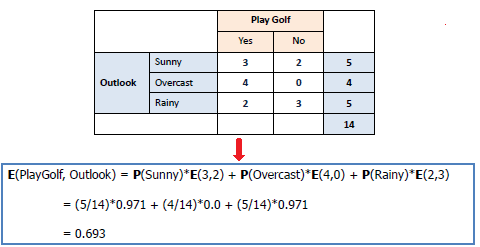
\includegraphics[width=10cm]{./img/07/entropy.png}
 \caption{\label{pic:entropy} Example of entropy calculation.}
\end{figure}






%========================================
\subsubsection{Random Forest}

A common problem when trying to build a model is to select significant features between all the available one. We tend to think that \textit{the more we have, the better it is}, even knowing the existence of the curse of dimensionality. 

Random Forest takes this idea and try to automatize this feature selection by randomly selecting subset of features.

The main idea of Random Forest algorithm is to grow an arbitrary number of \textbf{Decision Trees}, each one grown based on a subset of m features, randomly chosen between the total $p$ of them. It's an example of a \textbf{weak learner} saw in the Ensemble method. This weak learner has a lower bias (because of lower number of feature).

Following the \textbf{Ensemble method}, the predictions of all these weak learners are then merged together to produce a final prediction (by majority voting for example).



\begin{center} %---------------TAB--------------
\begin{tabular} {| l | l |}
\hline
\bf Pros & \bf Cons \\ \hline
+ Popular & - Not state-of-the-art  \\
+ Easy to implement & - Needs many passes over the data \\
+ Easy to parallelize & - Tend to overfit \\ 
\hline
\end{tabular}
\end{center}

%===============================
\subsubsection{Boosted Decision Trees}
Variante of Random Forest. Instead of training all DT independently on weak subset, the DT are trained sequentially and emphase incorrectly-labeled instances of the previous tree. This is called \textbf{Boosting}. 
\begin{itemize}
\item Low variance, because of the small trees handling small numbers of features
\item Low bias, reduces by the boosting
\end{itemize}

Opposed to RF that usually trained tens of medium-sized trees, BDT works on smaller trees in greater numbers.

Even if they show good results, their big drayback is their slow execution compared with the parallelized RF.

%===============================
\subsubsection{About model transparency}

A recurrent argument of using Decision Tree (DT) or Random Forest (RF) in industry is their transparency compared to state-of-the-art Deep-Neural-Network (DNN). This argument must be carefully taken. Even if by their very nature DT are more understandable by a human than DNN, the more features and Trees we had, the more complicated it becomes. Figure \ref{pic:RF_BT} shows the size of a common industry implementation of RF and BT where there are no more possibilities of human understanding.

\begin{figure}[H]%---------------FIG--------------
 \centering
 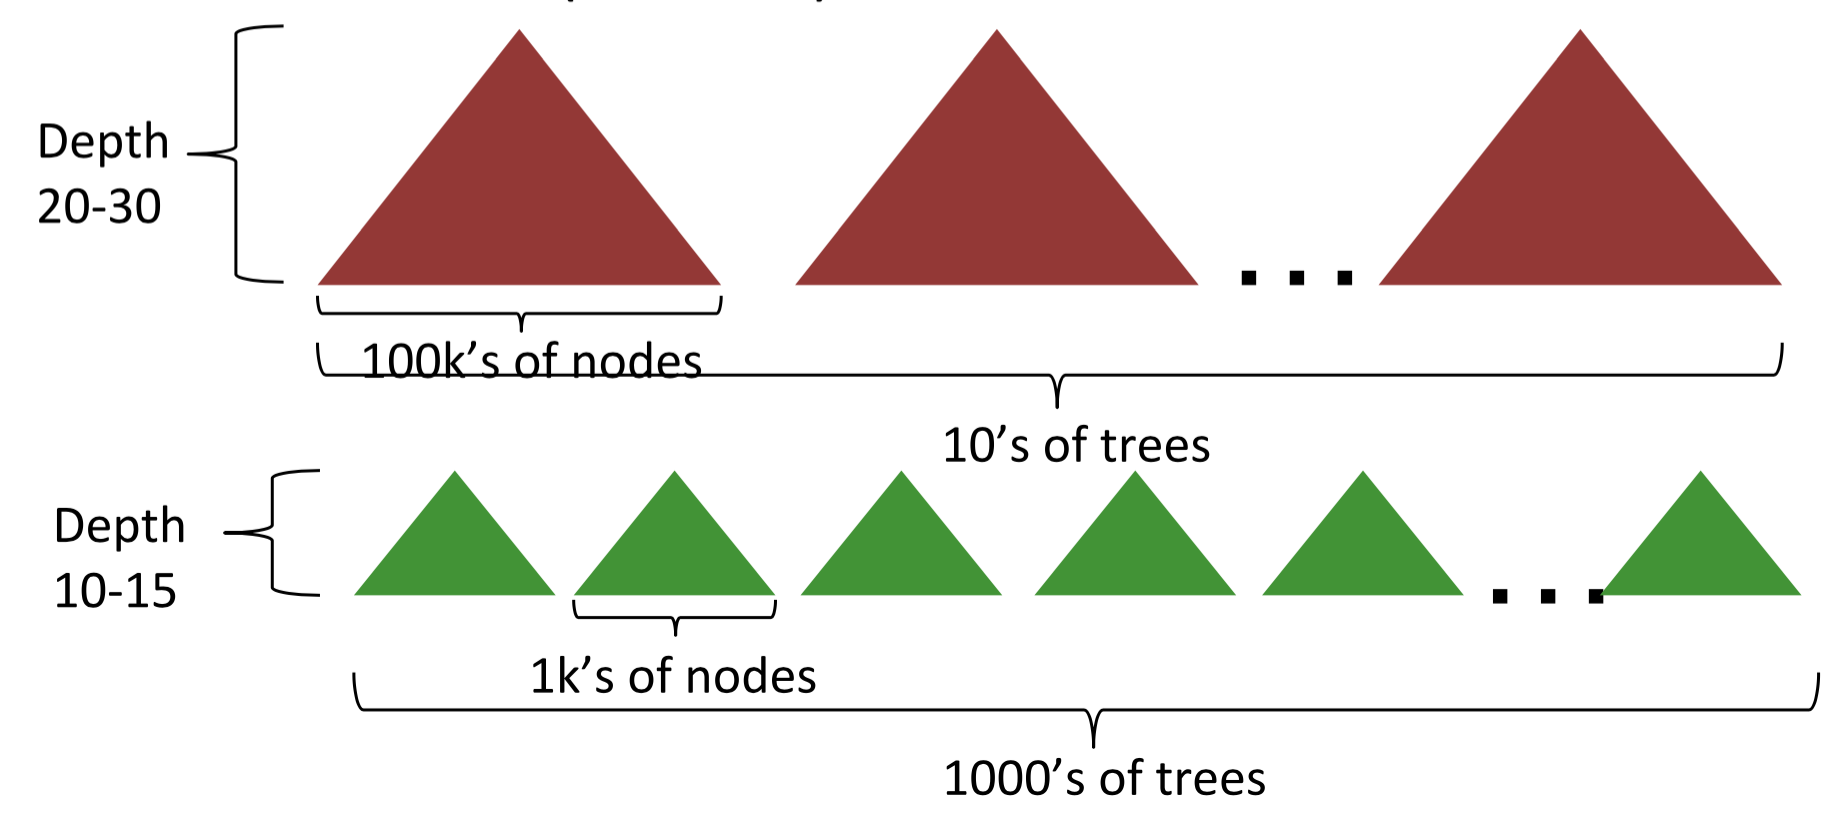
\includegraphics[width=10cm]{./img/07/RF_BT.png}
 \caption{\label{pic:RF_BT.} Standard size of RF and BDT implementations.
 In red: RF with big parallel DT. In green: BDT pipeline with lot of small DT}
\end{figure}


\subsection{Linear Regression}

Linear regression model produces a prediction equation:

$$
\hat{y} = \hat{\beta_0} + \sum\limits_{j=1}^p  X_j + \hat{ \beta_j}
$$

or in matrix notaction

$$
\hat{y} =X \hat{ \beta}
$$

Where $X_j$ are the data and $\hat{\beta_j}$ the characteristic of the model. 

\subsubsection{Statistic validation}

As a linear model can be calculated for every possible existing dataset, it is not enough to calculate it, but the existing of linear relationship between the data must be prooved.

\paragraph{$R^2$-value}

$R^2$-value describes how much of the total variance is reduced when we include the line as an offset. It computes the distances between the real $y$ and the predicted $\hat{y}$, and compares them with the distance between real $y$ and the mean $\bar{y}$.

\begin{itemize}
\item if $R^2 = 0$, then there is no difference between the linear model and the trivial mean $\bar{y}$. Then we conclude that there is not any evidence of linear relationship in our dataset and \textbf{we cannot use the model}.
\item if $R^2 = 1$, then the data perfectly alligned on the linear regression line and \textbf{the model is perfect}.
\end{itemize}

\begin{figure}[H]%---------------FIG--------------
 \centering
 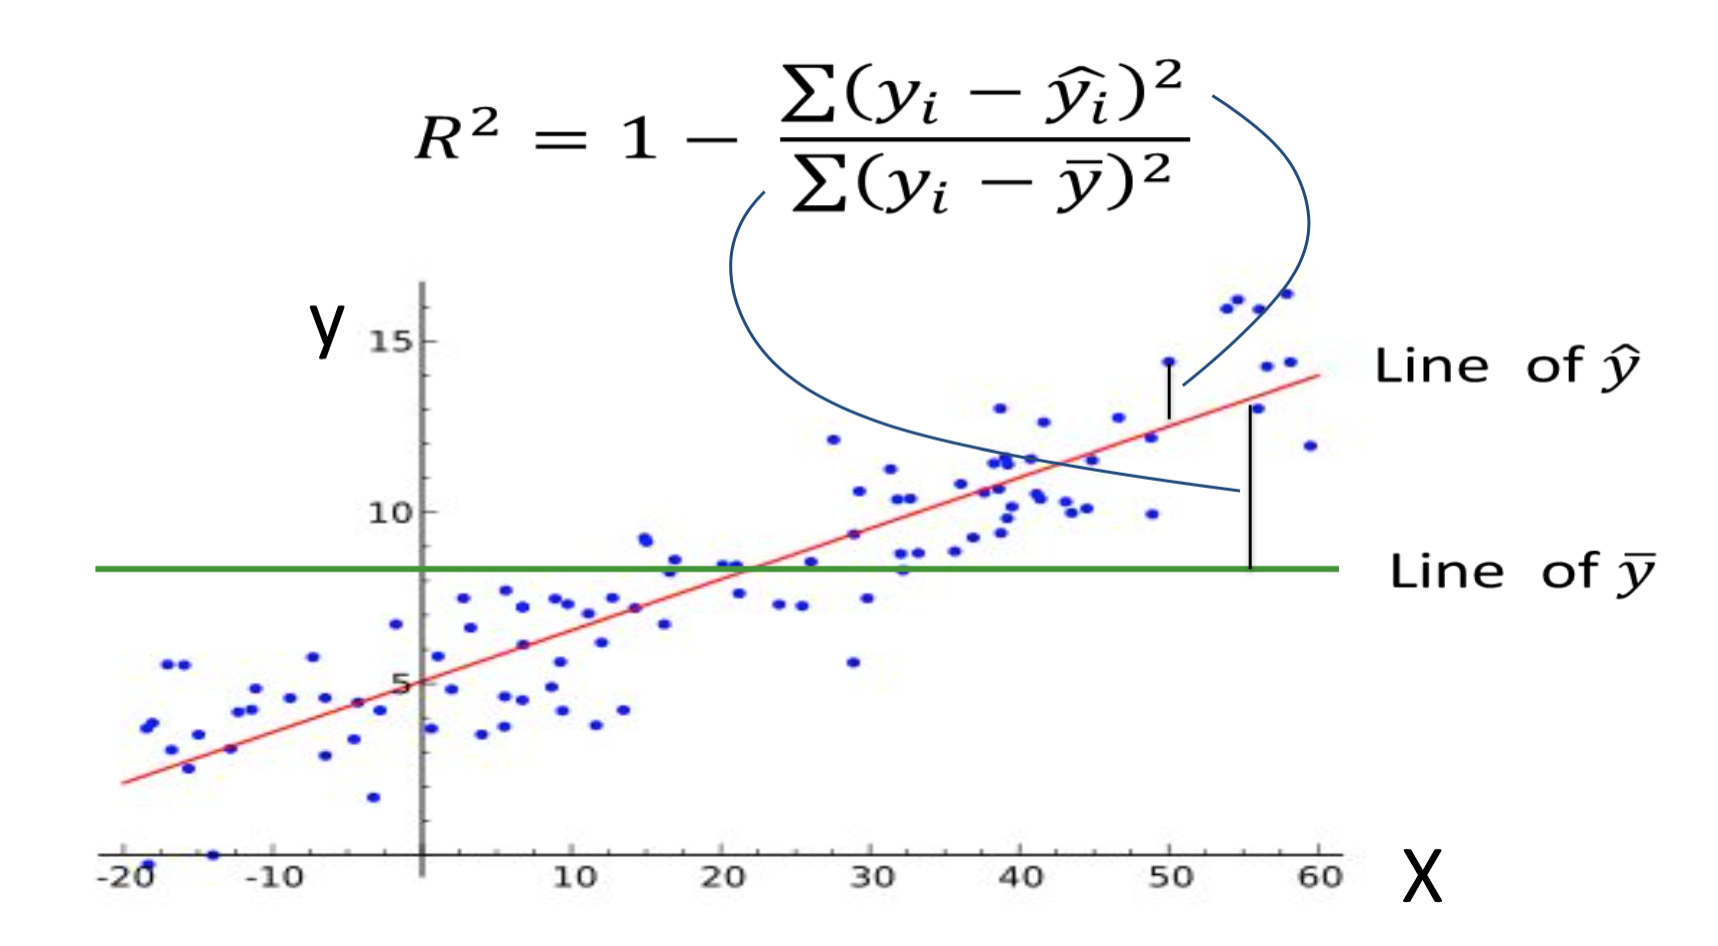
\includegraphics[width=10cm]{./img/07/r_2.png}
 \caption{\label{pic:r_2} Graphical meaning of $R^2$-value.}
\end{figure}


\paragraph{p-value}

From the Distribution of Fisher (F-Distribution) we can derive a p-value which is, as usual, the probability that the observed data are produced by the null hypothesis which is, in our case, the hypothesis \textit{no linear relationship}. For $p < 0.05$ we conclude, as usual, that it is very unlikely that the data were produced by the null hypothesis and we then accept the hypothesis \textit{the data are produced by linear relationship}.














